\section{Results}
\label{sec:results}

We report paired results on the \texttt{L1--L5} benchmark family for the five active ablations from Section~\ref{sec:agents}. The discussion moves from the average cross-model comparison to a selected layered read and then to behavior across the ladder.

\subsection{Cross-model comparison on the average ladder}

Figure~\ref{fig:results-model-ablation} shows the main average comparison. On the end-to-end \texttt{llm\_raw} condition, performance ranges from \texttt{0.697} directed F1 for \texttt{GPT-5.5} down to \texttt{0.113} for \texttt{Haiku-4.5}, with \texttt{Sonnet-4.6} at \texttt{0.314}, \texttt{Gemini-3-Flash} at \texttt{0.281}, and \texttt{GPT-5.4-mini} at \texttt{0.145}. \texttt{GPT-5.5} and \texttt{Sonnet-4.6} lead on SHD as well (\texttt{6.3} and \texttt{12.3}), but the bottom three flip places under SHD --- \texttt{Haiku-4.5} (\texttt{18.9}) and \texttt{Gemini-3-Flash} (\texttt{19.3}) sit below \texttt{GPT-5.4-mini} (\texttt{22.4}) because the smaller models submit fewer edges and accumulate fewer extra-edge errors at low directed F1.

\begin{figure}[!htbp]
\centering
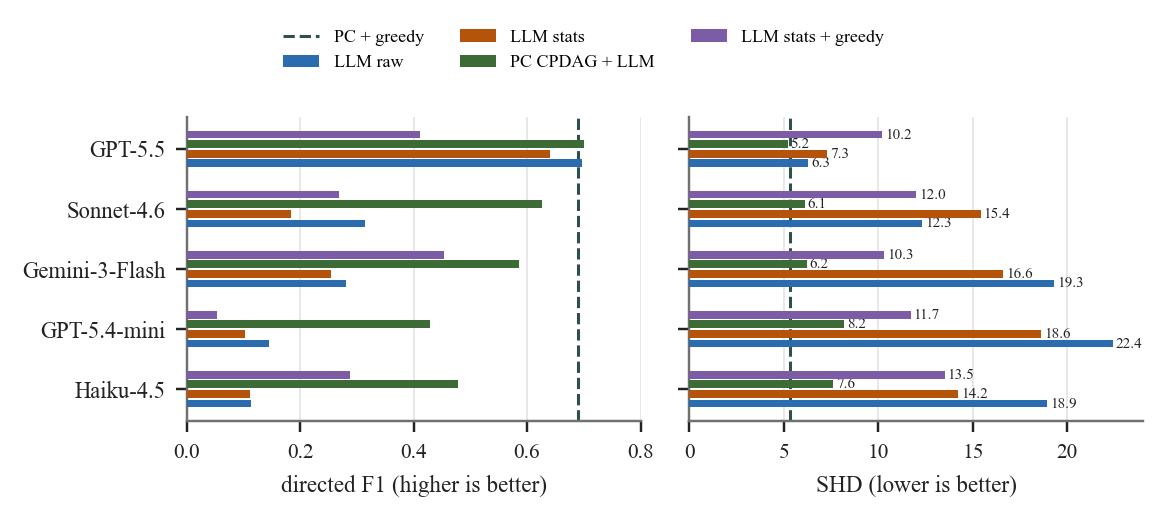
\includegraphics[width=\linewidth]{figures/generated/fig_results_model_ablation_v2.png}
\caption{Only \texttt{GPT-5.5} keeps pace with \texttt{pc\_greedy} (dashed) on end-to-end \texttt{llm\_raw}; the four weaker models close most of the gap once supplied with the PC-derived CPDAG (\texttt{pc\_cpdag\_llm}, green), while statistical-tool access alone (\texttt{llm\_stats}, orange) sits below \texttt{llm\_raw} for every model. Average over \texttt{L1--L5}.}
\label{fig:results-model-ablation}
\end{figure}


The same figure also makes the ablation pattern visible. Relative to \texttt{llm\_raw}, supplying the PC-derived CPDAG yields large directed-F1 gains for \texttt{GPT-5.4-mini} (\texttt{+0.284}), \texttt{Sonnet-4.6} (\texttt{+0.312}), \texttt{Haiku-4.5} (\texttt{+0.366}), and \texttt{Gemini-3-Flash} (\texttt{+0.304}), while the gain for \texttt{GPT-5.5} is only \texttt{+0.004}. By contrast, \texttt{llm\_stats} remains below \texttt{llm\_raw} for all five models. Across the current ladder, the larger variation comes from model capability and from the structural-prior cut rather than from adding CI-style statistical actions alone. Full per-model average tables across all five layered metrics are in Appendix~\ref{app:results:per-model}.

\subsection{Selected layered-score comparison}

Table~\ref{tab:results-layered-gpt55} gives one layered read over the strongest model. The end-to-end \texttt{llm\_raw} policy is nearly tied with \texttt{pc\_greedy} on directed F1 (\texttt{0.697} vs \texttt{0.689}), but the same comparison differs on both \texttt{comp\_f1} (\texttt{0.732} vs \texttt{0.612}) and SHD (\texttt{6.3} vs \texttt{5.3}). The scores therefore separate different error profiles rather than collapsing them into one ranking.

\begin{table}[tbp]
\centering
\caption{Selected \texttt{GPT-5.5} average \texttt{L1--L5} results. Higher is better for \texttt{skel\_f1}, \texttt{comp\_f1}, and \texttt{dir\_f1}; lower is better for \texttt{SHD}.}
\label{tab:results-layered-gpt55}
\scriptsize
\setlength{\tabcolsep}{4.0pt}
\begin{tabular}{lcccc}
\toprule
Policy & \texttt{skel\_f1} & \texttt{comp\_f1} & \texttt{dir\_f1} & \texttt{SHD} \\
\midrule
\texttt{pc\_greedy}     & 0.780 & 0.612 & 0.689 & 5.3 \\
\texttt{pc\_cpdag\_llm} & 0.789 & 0.615 & 0.701 & 5.2 \\
\texttt{llm\_raw}       & 0.753 & 0.732 & 0.697 & 6.3 \\
\texttt{llm\_stats}     & 0.704 & 0.673 & 0.640 & 7.3 \\
\bottomrule
\end{tabular}
\end{table}

The same slice also clarifies the stronger ablation. \texttt{pc\_cpdag\_llm} slightly improves both directed F1 and SHD relative to \texttt{pc\_greedy}, while keeping the CPDAG-facing scores close. In this setting, supplying the observational structure changes the comparison from end-to-end discovery to final orientation quality. That is the narrowest place in the paper where the strongest model comes close to the classical active baseline, and it is best read as a secondary observation rather than the headline. The same layered breakdown for the other four models is in Appendix~\ref{app:results:per-model}.

\subsection{Behavior across the ladder}

The gap also widens as the accepted instances become harder. The classical \texttt{pc\_greedy} baseline drops from \texttt{0.802} at \texttt{L1} to \texttt{0.642} at \texttt{L5} (\texttt{-0.160}). Over the same range, \texttt{llm\_raw} drops from \texttt{0.824} to \texttt{0.537} for \texttt{GPT-5.5} (\texttt{-0.287}), from \texttt{0.426} to \texttt{0.252} for \texttt{Sonnet-4.6} (\texttt{-0.174}), from \texttt{0.414} to \texttt{0.185} for \texttt{Gemini-3-Flash} (\texttt{-0.229}), and from \texttt{0.192} to \texttt{0.047} for \texttt{Haiku-4.5} (\texttt{-0.145}, but starting near the floor with little room to fall further). On the reported \texttt{L1--L5} family, the four \texttt{llm\_raw} runs that start at non-trivial directed F1 at \texttt{L1} therefore lose more across the ladder than the classical active baseline does, while \texttt{Haiku-4.5} sits near the floor throughout. The full per-level $\times$ per-model breakdown across all policies is in Appendix~\ref{app:results:per-level}, and trace-level views of representative successes and failures behind these averages are in Appendix~\ref{app:traces}.

\FloatBarrier
